\section{Call-matched accuracy, cost and signal sensitivity}\label{sec:call}
The MATH-500 data contribute 45,000 published grades; the three chosen AIME models contribute 360. All selected question--model cells contained the required distinct positions. Table~\ref{tab:sample} reports the calibration split and the resulting test-set call rates. The six AIME calibration questions make the observed upgrade rate especially sensitive to the chosen threshold. Each dataset's shared fallback or first stage induces dependence between its configurations.

\begin{table}[htbp]\centering\small
\caption{Frozen length gates. Cutoffs are recorded first-stage output tokens; calls are the fraction upgraded on evaluation questions. Accuracy columns give standalone first-stage and fallback percentages. The 1.5B token signal has missing telemetry.}\label{tab:sample}
\begin{tabular}{lrrrrr}
\toprule
Configuration & Cal./eval. & Draws & Cutoff & Calls & First / fallback \\
\midrule
Nano to Super & 100/400 & 30 & 3,379 & 24.7\% & 96.8 / 96.6 \\
Nano to Llama & 100/400 & 30 & 3,379 & 24.7\% & 96.8 / 76.1 \\
1.5B to 32B & 6/24 & 4 & 18,883 & 37.5\% & 18.8 / 60.4 \\
14B to 32B & 6/24 & 4 & 17,993 & 19.8\% & 50.0 / 60.4 \\
\bottomrule
\end{tabular}

\end{table}

\paragraph{A narrow accuracy finding on MATH-500.}
Nano and Super had similar standalone performance. Under independent within-question pairing, the gate gained 0.164 points over random escalation at the same 24.7\% call rate. Targeting within-question failures contributed 0.026 points; assigning different call rates across questions contributed 0.138. A model-wide change of run labels could shrink the accuracy lead to 0.010 points. Question-specific relabeling extended the lower endpoint to $-0.007$ points, a practically negligible adverse value. Fourteen of the 400 questions sufficed to erase the identity result, and 13 could not. The gate itself varied across draws on 137 questions. Uniform permutations had a standard deviation of about 0.020 points under either convention. An adversarial edge near zero and a typical perturbation near the product value describe different properties of the same archive.

\begin{table}[htbp]\centering\footnotesize
\caption{Accuracy difference against the call-matched random comparator, in percentage points. ID uses the archived replicate position. The two SDs refer to uniform common and question-specific permutations. Erase counts the fewest individually rematched questions needed to reach the opposite weak sign from ID. Infinity means no such rematching exists.}\label{tab:acc}
\begin{tabular}{lrrrrrr}
\toprule
Configuration & ID & Product & Common & Per question & SDs & Erase \\
\midrule
Nano to Super & 0.15 & 0.16 & [0.01, 0.31] & [-0.01, 0.33] & 0.02/0.02 & 14 \\
Nano to Llama & -8.54 & -8.53 & [-9.06, -7.95] & [-9.96, -7.35] & 0.06/0.06 & $\infty$ \\
1.5B to 32B & 7.29 & 4.95 & [2.08, 7.29] & [0.00, 11.46] & 1.42/1.63 & 7 \\
14B to 32B & 3.15 & 4.19 & [3.15, 6.27] & [0.02, 7.31] & 0.85/1.20 & $\infty$ \\
\bottomrule
\end{tabular}

\end{table}

Switching only the fallback to Llama produced an 8.527-point loss under independent pairing. Every reindexing preserved its sign. The within-question targeting term was identical because it depends only on the first-stage answers. The marked difference arose from the allocation of extra calls to questions on which Llama performed poorly relative to Nano. Table~\ref{tab:controls} separates both effects and gives the comparisons with fixed policies.

\paragraph{Cost changes the primary result.}
Despite equal expected fallback call counts, sending long Nano responses to Super also selected questions whose Super responses were long. The product contrast added 1,142 Super output tokens per incoming request. Even the least expensive question-specific alignment added 1,024. At a penalty of 0.1 accuracy points per 1,000 tokens, product utility was $+0.050$ points and its common-alignment range straddled zero. At a penalty of one point, even the most favorable question-specific match yielded $-0.702$ points. Figure~\ref{fig:align} contrasts this with the positive product estimate on AIME. For the stronger AIME first stage the common-alignment utility range was $[1.61,5.09]$, while the question-specific range was $[-1.86,6.79]$. Simply combining the worst marginal accuracy and maximum marginal cost would give $-2.09$ rather than the attainable $-1.86$.

\begin{figure}[htbp]\centering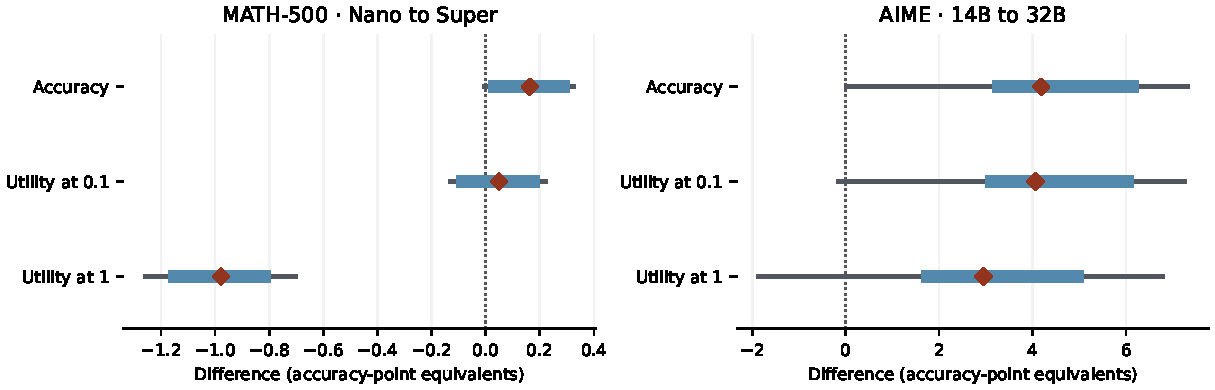
\includegraphics[width=.97\linewidth]{alignment.pdf}
\caption{The length gate minus the call-matched random gate. Thin lines mark question-specific extrema, thick segments mark common extrema, and diamonds mark product pairing. Utility penalties are accuracy points per thousand extra fallback output tokens. The panels use different horizontal scales.}\label{fig:align}
\end{figure}

\paragraph{A pre-answer random comparator can skip work.}
A random router can bypass the first model on requests it escalates. A streaming gate can discard its first response when it observes token $T+1$. With immediate cancellation its first-stage output cost is $\min(L,T+1)$, against $(1-r)L$ in expectation for random bypass. Add this identified first-stage difference to $\rho$ times the aligned fallback-token difference, where $\rho$ is the fallback price relative to the first-stage price per output token. On Nano to Super, the gate saved 183 first-stage tokens per request but still consumed at least 841 additional price-weighted tokens at $\rho=1$. In the Llama comparison the entire cost interval changed sign between $\rho=1$ and $4$, despite an accuracy loss under both. These are counterfactual output-accounting examples conditional on immediate cancellation and full access to emitted tokens.

\begin{table}[htbp]\centering\footnotesize
\caption{Streaming length gate versus pre-answer random bypass. All columns are per incoming request. The fallback point uses the product pairing. Ranges permit question-specific reindexing. The last two columns are weighted token differences in first-stage equivalents. Missing 1.5B telemetry precludes this comparison.}\label{tab:cost}
\begin{tabular}{lrrrrr}
\toprule
Configuration & $\Delta$ first & $\Delta$ fallback & Fallback range & $\rho=1$ & $\rho=4$ \\
\midrule
Nano to Super & -183 & 1142 & [1024, 1255] & [841, 1072] & [3914, 4838] \\
Nano to Llama & -183 & 102 & [78, 131] & [-105, -53] & [129, 339] \\
14B to 32B & 1442 & 1237 & [405, 2109] & [1846, 3551] & [3060, 9878] \\
\bottomrule
\end{tabular}

\end{table}

\paragraph{Independent archive and data audit.}
On the AIME 14B-to-32B pair, all 24 common column permutations favored the recorded-length gate in accuracy. It gained 4.188 points under independent pairing. Even the worst question-specific match retained a small positive margin of 0.022 points. Only two rematched questions could erase its identity-match utility advantage at the one-point penalty. Large favorable accuracy estimates alone give little information about the stability of a cost-sensitive decision.

For the 1.5B first stage, 45 of 120 records had zero recorded output tokens despite containing nonempty answer text, including 11 archived correct responses. Treating the recorded number as the signal is a reproducible audit of that field, but it invalidates a literal interpretation as elapsed generation length. We retain the original analysis in the tables for traceability. We excluded this pair from the streaming cost comparison and repeated both AIME gates using the observed number of Unicode code points in each released answer. We retained the original calibration and test questions, fallback costs and labels. This sensitivity was designed after finding the telemetry problem.
For 1.5B, the character gate escalated 20.8\% of requests at a cutoff of 94,336 characters. Its product accuracy gain was 3.04 points and its common range was $[0.69,4.86]$; the question-specific range $[-1.39,7.99]$ admitted a loss. With 14B first, the cutoff was 1,679 characters, the call rate 24.0\%, and the product gain only 0.89 points. Six of the 24 common permutations favored random escalation, whereas all 24 had favored the token gate. Its question-specific range was $[-3.54,5.84]$. This is a reversal under a simple global change of index convention. Released answer-text length and recorded generation-token usage are different observable signals; the released fields do not establish which generated tokens were displayed. Neither signal can be universally substituted for the other.


\begin{table}[htbp]\centering\footnotesize
\caption{Product accuracy comparisons in points. Keep, Median and Always are alternative fallback rules. Within and Between decompose the primary contrast. The last column repeats that contrast using all questions with the same previously fitted cutoff.}\label{tab:controls}
\begin{tabular}{lrrrrrr}
\toprule
Configuration & Keep & Median & Always & Within & Between & All questions \\
\midrule
Nano to Super & 0.11 & 0.34 & 0.32 & 0.03 & 0.14 & 0.21 \\
Nano to Llama & -13.66 & 5.14 & 7.09 & 0.03 & -8.55 & -7.86 \\
1.5B to 32B & 20.57 & -11.20 & -21.09 & 0.52 & 4.43 & 4.33 \\
14B to 32B & 6.25 & -1.56 & -4.17 & 3.39 & 0.80 & 5.66 \\
\bottomrule
\end{tabular}

\end{table}
